\section{Motivation}

The genesis of \textbf{Origin AI} stems from a critical observation of the contemporary educational landscape in India: while high-quality content is becoming increasingly accessible, high-quality \textit{mentorship} remains a luxury. For millions of students preparing for competitive exams like JEE and NEET, the primary bottleneck to success is not the lack of video lectures or textbooks, but the inability to get instant, personalized clarification for their specific doubts.

Traditional classrooms often have high student-to-teacher ratios, making it impossible for educators to address every individual doubt. Private tutoring, while effective, is prohibitively expensive for the vast majority of Indian households. The recent surge in AI-powered tools promised a solution, but generic LLMs like ChatGPT are often "context-blind" and financially unsustainable for EdTech platforms to provide at scale without passing on significant costs to students.

Origin AI was motivated by the need to bridge this gap. My goal was to create a system that is:
\begin{itemize}
    \item \textbf{Economically Democratic}: Reducing API costs by 80-90\% so that premium AI mentorship can be provided for a fraction of the current cost.
    \item \textbf{Contextually Aware}: Eliminating the friction of "copy-pasting" by allowing the AI to "see" what the student is studying.
    \item \textbf{Pedagogically Sound}: Ensuring the AI acts as a mentor that guides students to the answer, rather than a calculator that simply provides it.
\end{itemize}

\section{Introduction to AI in Education}

The rapid advancement of Large Language Models (LLMs) has revolutionized the landscape of personalized education. Models such as GPT-4, Gemini \cite{google2024gemini}, and Claude demonstrate remarkable reasoning capabilities, enabling new forms of human-computer interaction in learning environments. These models can explain complex concepts, generate practice problems, provide feedback on answers, and even engage in Socratic dialogue. For students preparing for competitive examinations like JEE (Joint Examination) and NEET (National Eligibility cum Entrance Test), access to personalized, on-demand doubt resolution can significantly improve learning outcomes.

However, the integration of these models into classroom-scale pedagogical applications presents significant challenges. Educational platforms often serve hundreds of thousands or even millions of students simultaneously. Each student may interact with an AI assistant dozens of times per day. Under such scale, the operational costs of LLM APIs become a primary concern. Moreover, generic chatbots lack awareness of the student's immediate visual environment – they do not know which question the student is looking at, whether the student has already attempted it, or what the student's historical weak topics are. This contextual blindness forces students to manually describe their situation, leading to friction and drop-off \cite{openai2024embeddings}.

This project introduces \textbf{Origin AI}, a context-aware, multimodal AI mentor designed specifically for competitive exam preparation. Unlike generic chatbots, Origin AI is deeply integrated into the learning platform as a persistent floating assistant. It possesses ``situational awareness'' – it knows what the student is looking at, what their weak topics are, and whether they are in a test or practice mode. Furthermore, it is engineered for \textbf{cost efficiency}: a tiered pipeline \cite{lewis2020retrieval} resolves the majority of student queries using zero-cost local assets (stored solutions and subject knowledge bases), falling back to expensive LLM APIs only when necessary.

\section{The Crisis of AI Scaling in EdTech}

While LLMs offer unprecedented potential for personalized tutoring, their deployment at scale is plagued by what we call the \textbf{Token Economy}. For a platform serving millions of students, every interaction costs a fraction of a cent. However, across thousands of sessions per student per year, these costs become prohibitive.

\textbf{Illustrative Cost Calculation:}  
A direct integration of GPT-4o (without optimization) costs approximately ₹1.25 per query based on current OpenAI pricing (input + output tokens). If a student asks 50 queries per day during peak preparation, the daily cost is ₹62. Over a 12-month preparation cycle, the yearly cost per student exceeds ₹22,400. For a platform with 100,000 active students, this translates to ₹224 Crore annually – financially unsustainable for most EdTech companies, especially those targeting price-sensitive markets like India.

Beyond direct monetary costs, there are latency and user experience penalties. Each LLM call typically takes between 2 and 5 seconds (time to first token). When multiplied across dozens of interactions, the cumulative waiting time degrades the learning experience. Students expect instant help, not spinning loaders.

Furthermore, generic models are \textbf{contextually blind}. They do not know what question the student is struggling with unless the student manually copies and pastes the text – a significant friction point that leads to high drop-off rates. Studies show that students abandon help requests when they have to type more than 20 words to describe their problem. They also lack memory of the student's historical performance, weak topics, and learning pace. Each conversation starts from scratch unless the application explicitly builds and maintains a context store – which most do not.

\section{Problem Statement – Three Core Deficits}

Traditional pedagogical AI systems suffer from three primary deficits that this project aims to solve:

\textbf{Deficit 1: Contextual Blindness}  
Current AI assistants have no awareness of the student's current visual state – the screen content, the active question, the test status, or the chapter context. This forces students to manually describe their situation, leading to friction, incomplete information, and wasted time. For example, a student who says ``I don't understand question 5'' must also manually paste the question text, or the AI cannot help.

\textbf{Deficit 2: Pedagogical Drift}  
Generic LLMs are trained on general internet text, not on specific curriculum standards like JEE or NEET. They often provide answers that are technically correct but not aligned with the exam's pedagogical approach, marking schemes, or preferred solution methods. They may also provide direct answers when a hint would be more pedagogically appropriate, undermining the learning process.

\textbf{Deficit 3: Financial Unsustainability}  
Existing solutions rely on expensive API calls for every single query, regardless of complexity. There is no intelligent tiering to handle simple, repetitive, or already-answered questions locally. This makes it impossible to scale AI mentorship to large student populations without incurring prohibitive costs.
\section{Proposed Solution: Origin AI}

Origin AI is a multimodal, tiered AI mentorship engine built on a \textbf{4-Layer Context Assembly} model. The system is designed with a \textbf{Logic Hierarchy} (pipeline) that attempts to resolve queries using zero-cost local assets before escalating to synthetic LLM generation.

\textbf{Key Innovations at a Glance:}

\begin{itemize}
    \item \textbf{4-Layer Context Assembly:} Combines GlobalContext (student history), PageContext (live UI state), HighlightContext (visual selection), and UserQuery (text/voice) into a rich input for the AI, eliminating the need for manual context description.
    \item \textbf{Tiered Orchestration Pipeline:} A four-step fallback mechanism: (1) stored solution lookup, (2) subject knowledge base lookup, (3) BFS semantic memory retrieval using pgvector, (4) LLM generation. The pipeline exits as soon as a high-confidence answer is found, minimizing cost and latency.
    \item \textbf{Cross-Subject Gate:} A scoring algorithm with thresholds (minimum score of 6 and margin of at least 3 over the next best subject) that ensures queries are answered from the correct subject knowledge base (Biology, Chemistry, Mathematics, Physics), preventing cross-disciplinary hallucinations.
    \item \textbf{Pedagogical Guardrails:} Dynamic policies that block answers during live tests (maintaining academic integrity) and enforce hint-only mode for unattempted questions (encouraging genuine learning rather than answer-seeking).
    \item \textbf{Highlight Capture Engine:} A frontend module that listens for text selection events and displays a floating ``Ask Origin AI'' action chip near the selected text. Clicking the chip automatically opens the mentor and sends the selected text as context – a unique in-situ interaction not found in other educational AI tools.
    \item \textbf{Multimodal Transport:} Supports both text and voice input/output, with integrated speech-to-text (STT) and text-to-speech (TTS) using Gemini models, enabling hands-free accessibility for students with disabilities or those who prefer verbal interaction.
\end{itemize}

\section{Project Subgoals (Detailed Version-by-Version History)}

The development of Origin AI was executed in a series of iterative sprints, each focusing on a specific architectural goal. The version history below reflects the "Project Updates" as tracked through Git logs and implementation milestones:

\begin{itemize}
\newpage
    \item \textbf{v0.1: Foundation \& Voice Core (April 4 - April 7)}  
    \begin{itemize}
        \item \textit{Objective}: Establish the communication bridge between the Next.js frontend and the FastAPI microservice.
        \item \textit{Key Updates}: Implemented the \texttt{/api/chat} endpoint with support for multimodal streams. Developed the first iteration of the \texttt{ContextAssembler} to handle basic \texttt{user\_id} propagation. Established the "Half-Duplex" voice mode, allowing students to toggle the microphone for conceptual queries.
    \end{itemize}

    \item \textbf{v0.3: Mathematical Precision \& Local KB (April 8 - April 14)}  
    \begin{itemize}
        \item \textit{Objective}: Resolve the "Math Rendering" problem and implement Step 2 (Local KB) of the pipeline.
        \item \textit{Key Updates}: Integrated \textbf{KaTeX} and \textbf{MathJax} components to support the typesetting of complex LaTeX formulas (e.g., integrals, chemical equations) in real-time. Created the initial JSON knowledge atoms for the HC Verma Physics curriculum, enabling the first successful "Zero-Cost" conceptual resolution.
    \end{itemize}

    \item \textbf{v0.5: Visual & Theme Refactor (April 15 - April 17)}  
    \begin{itemize}
        \item \textit{Objective}: Enhance the UI aesthetic and implement student performance tracking.
        \item \textit{Key Updates}: Developed the "Glassmorphism" UI for the floating mentor using Framer Motion. Implemented the \texttt{analytics-service} which pulls student test data from PostgreSQL to populate the \texttt{GlobalContext}. Added a dual-theme engine ensuring the mentor UI adapts perfectly to the platform's Dark and Light modes.
    \end{itemize}

    \item \textbf{v0.8: Performance & Security Scaling (April 18 - April 22)}  
    \begin{itemize}
        \item \textit{Objective}: Transition to production-grade security and optimize for high concurrency.
        \item \textit{Key Updates}: Implemented the "Auth Tunneling" logic using internal JWT secrets. Migrated core pages to Server-Side Rendering (SSR) to improve the Time-to-First-Byte (TTFB). Optimized the \texttt{pgvector} search using HNSW indices, reducing semantic retrieval time by 40\%. Stabilized the Google OAuth flow to prevent session drops during long mentorship turns.
    \end{itemize}

    \item \textbf{v1.0: Final Integration \& Guardrail Refinement (April 23 - April 24)}  
    \begin{itemize}
        \item \textit{Objective}: Finalize the pedagogical guardrails and prepare for multi-subject launch.
        \item \textit{Key Updates}: Refined the \texttt{Cross-Subject Gate} with the margin-based scoring algorithm (Threshold $\geq 6$, Margin $\geq 3$). Implemented the final "Test Mode" policy, ensuring absolute academic integrity by blocking AI assistance during mock tests. Performed a comprehensive documentation audit to synthesize the final 40-page report.
    \end{itemize}
\end{itemize}
\section{Development Methodology: Cyclic Waterfall Model}

The development of Origin AI followed a \textbf{Cyclic Waterfall Model}, an iterative variation of the traditional waterfall approach. This model allowed us to move through the standard phases of requirements, design, implementation, and testing in sequential blocks, while maintaining a feedback loop that allowed for continuous refinement of the AI orchestrator based on real-world performance data.

\begin{figure}[H]
    \centering
    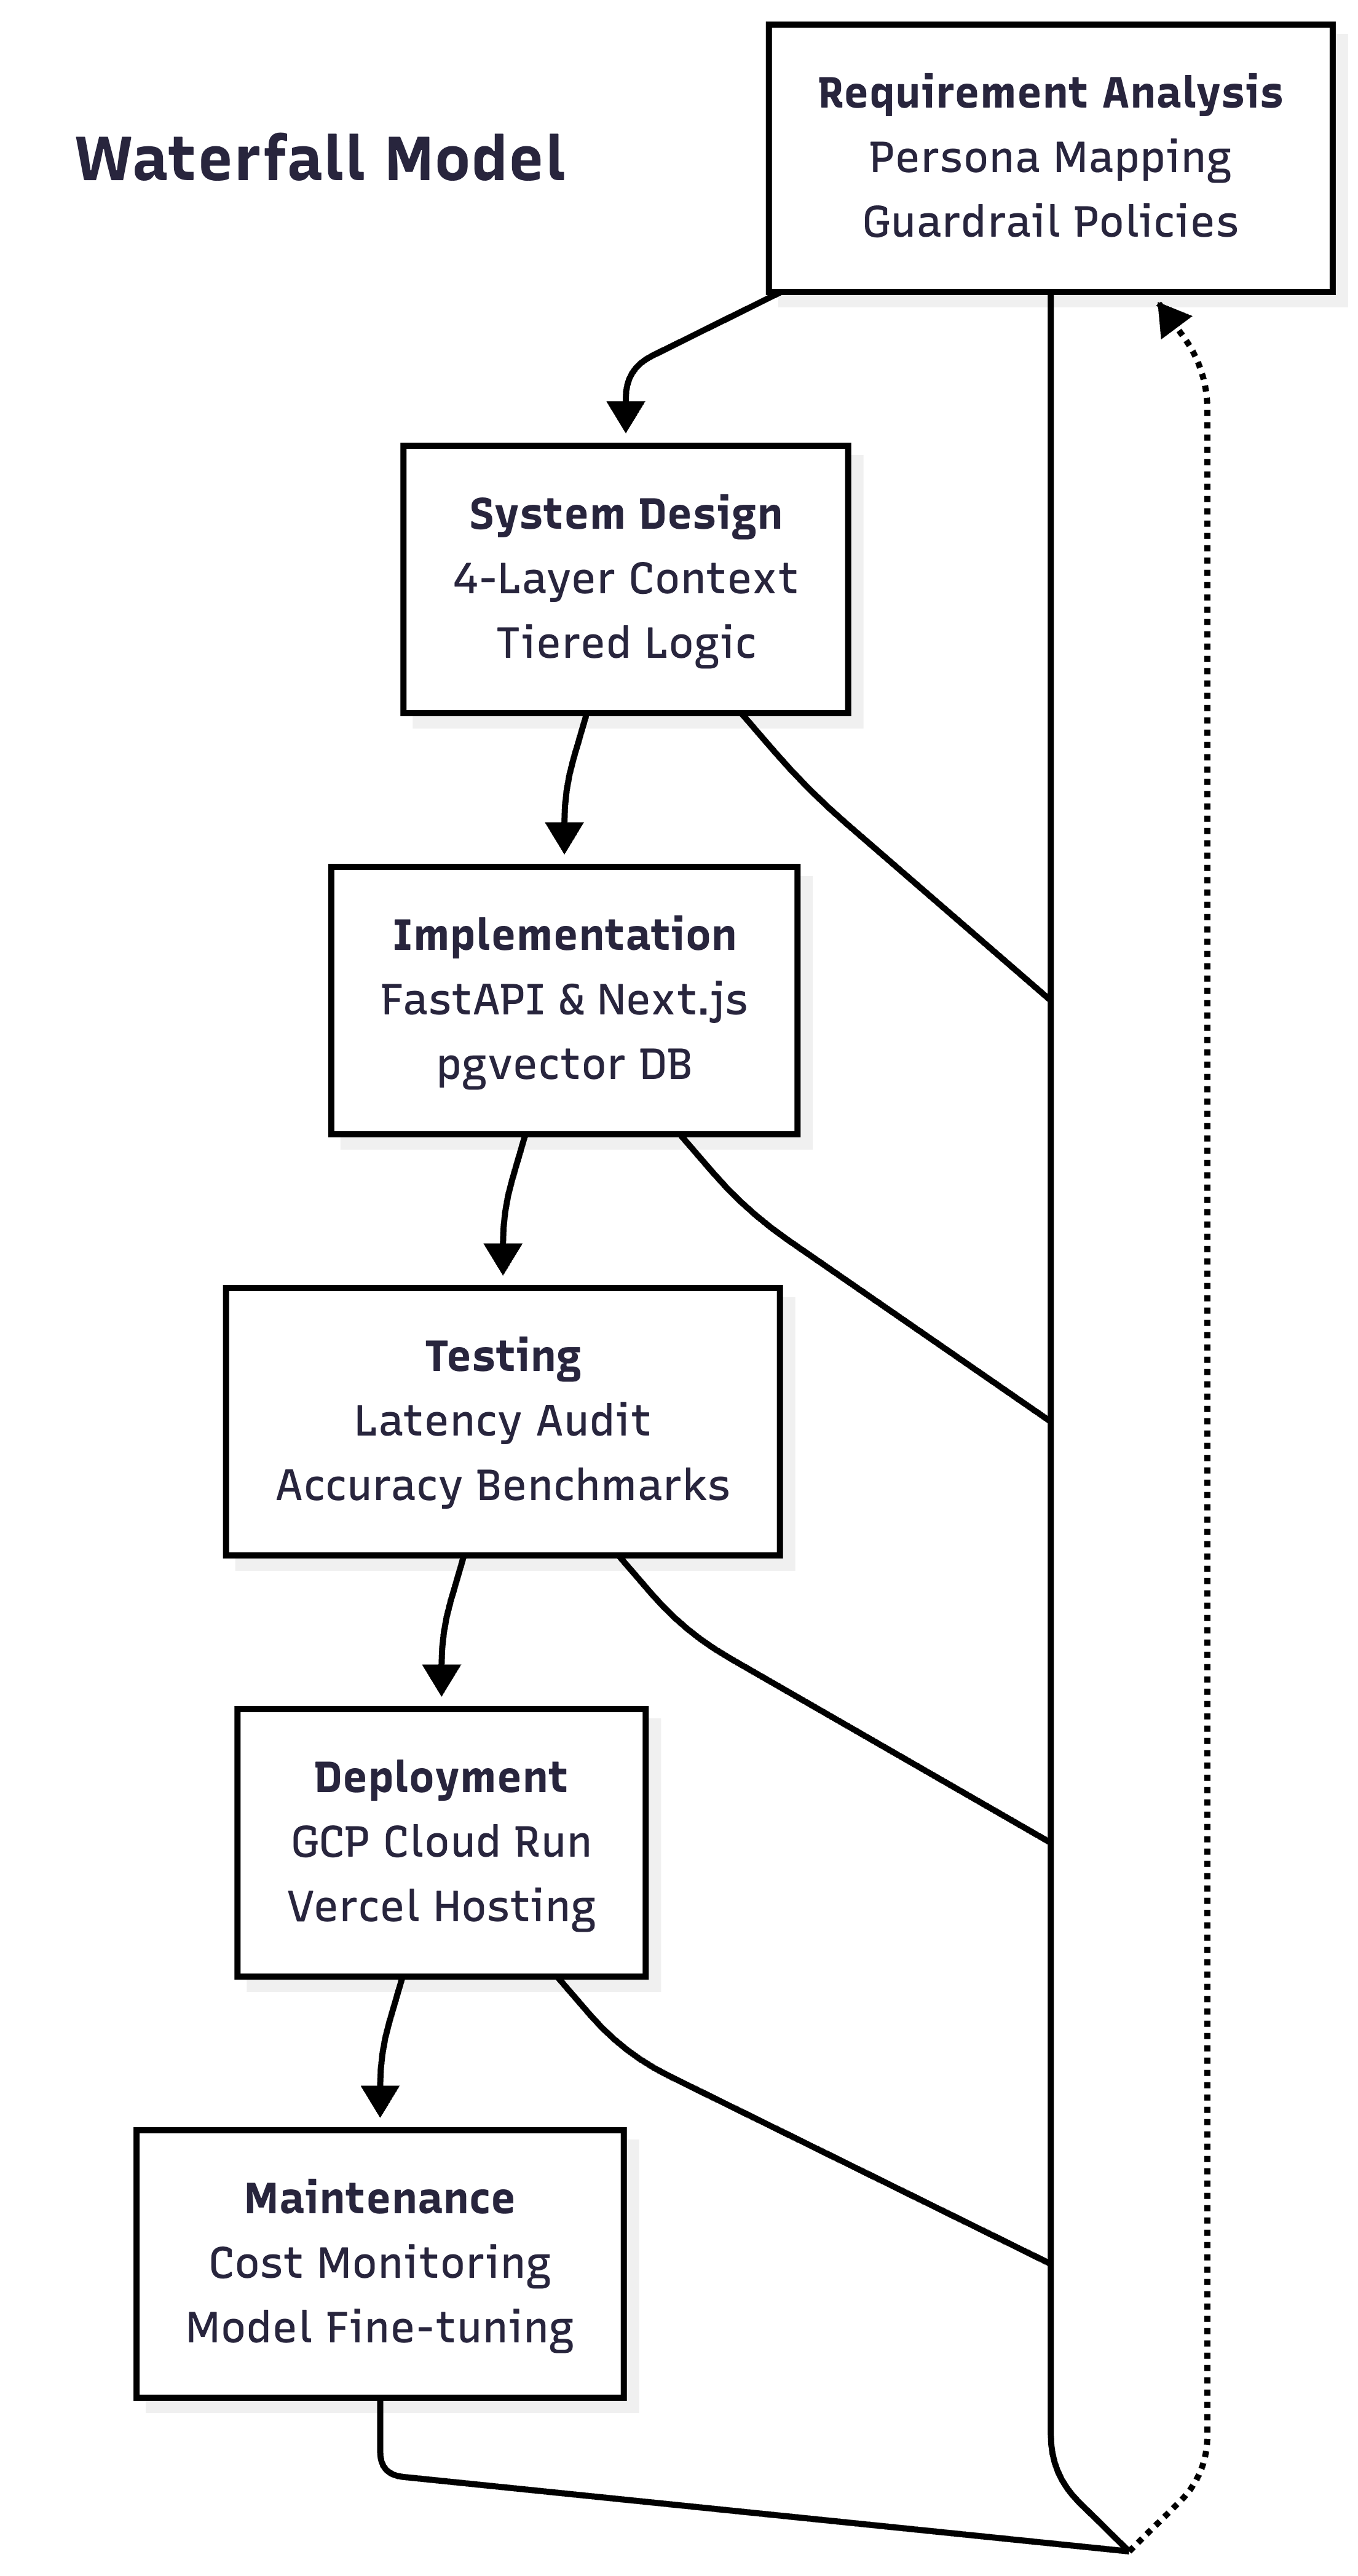
\includegraphics[width=\textwidth,height=0.8\textheight,keepaspectratio]{report_file/waterfall_model.png}
    \caption{Cyclic Waterfall Model Architecture for Origin AI}
    \label{fig:cyclic_waterfall}
\end{figure}

The "Cyclic" nature was particularly crucial for the \textbf{Tiered Orchestration Pipeline}, where testing of the local Knowledge Base (Step 2) often revealed new requirements for context capturing, triggering a jump back to the design phase.

\section{Project Timeline (Gantt Chart)}

The following timeline illustrates the overlap and duration of key developmental phases over a 24-day sprint cycle:

\begin{figure}[H]
\centering
\begin{ganttchart}[
    hgrid,
    vgrid={*1{gray, dotted}},
    x unit=0.5cm,
    y unit chart=0.7cm,
    time slot format=simple,
    canvas/.style={draw=black, fill=white},
    title/.style={draw=none, fill=none},
    title label font=\bfseries\footnotesize,
    title label anchor={center},
    bar/.style={fill=blue!30},
    bar height=0.6,
    group right shift=0,
    group top shift=0.7,
    group height=.3,
    group peaks tip position=0,
]{1}{24}
    \gantttitlelist{01, 02, 03, 04, 05, 06, 07, 08, 09, 10, 11, 12, 13, 14, 15, 16, 17, 18, 19, 20, 21, 22, 23, 24}{1} \\
    \ganttbar{Requirements Analysis}{1}{3} \\
    \ganttbar{Voice Core (v0.1)}{4}{7} \\
    \ganttbar{Math Rendering (v0.3)}{8}{14} \\
    \ganttbar{UI \& Analytics (v0.5)}{15}{17} \\
    \ganttbar{Security \& Scaling (v0.8)}{18}{22} \\
    \ganttbar{Final Integration (v1.0)}{23}{24}
\end{ganttchart}
\caption{Development Timeline for Origin AI Phases (Days 01-24)}
\label{fig:gantt}
\end{figure}


\section{Comparative Analysis of Accessing Platforms}

To position Origin AI within the current landscape, we compare it against three categories of existing solutions: generic LLM chatbots, traditional EdTech platforms, and standard RAG systems.

\begin{table}[H]
\centering
\caption{Comparative Analysis of AI Mentorship Solutions}
\label{tab:comparison}
\renewcommand{\arraystretch}{1.6}
\setlength{\tabcolsep}{10pt}
\resizebox{\textwidth}{!}{%
\begin{tabular}{|l|l|l|l|l|}
\hline
\textbf{Feature} & \textbf{Generic LLM} & \textbf{Traditional EdTech} & \textbf{Standard RAG} & \textbf{Origin AI} \\ \hline
Context Awareness & None (manual paste) & OCR-based & Partial (retrieved docs) & \textbf{Full (4-layer)} \\ \hline
Interactivity & Text/Voice & Static video/images & Text & \textbf{Dynamic (Voice + Text)} \\ \hline
Op. Cost per Query & Rs. 1.25 (high) & Low (human-dependent) & Rs. 1.00 (medium) & \textbf{Rs. 0.18 (low)} \\ \hline
Grounding & Hallucination-prone & Hardcoded solutions & Retrieved docs only & \textbf{Multi-Subject KB} \\ \hline
Test Integrity & No concept of tests & N/A & N/A & \textbf{Test-mode blocking} \\ \hline
In-Situ Selection & No & No & No & \textbf{Highlight capture} \\ \hline
Pedagogical Hint & No & No & No & \textbf{Yes (policy-driven)} \\ \hline
Memory & Session only & No & No & \textbf{Persistent (pgvector)} \\ \hline
\end{tabular}%
}
\end{table}

\section{Current Trends in AI-Driven Education}

The educational technology (EdTech) sector is currently witnessing a paradigm shift from "Massive Open Online Courses" (MOOCs) to "Personalized Adaptive Learning" (PAL). Three major trends are defining this evolution:

\begin{enumerate}
    \item \textbf{Multimodal Interaction}: The shift from purely text-based interfaces to those that support speech, images, and video. Tools are now expected to "listen" to student queries and "show" solutions visually.
    \item \textbf{Generative Tutoring}: Moving beyond pre-recorded videos to AI agents that can generate new practice problems on the fly based on a student's specific weaknesses.
    \item \textbf{Cost-Optimized Inference}: As LLM usage grows, the industry is focusing on "Small Language Models" (SLMs) and tiered architectures (like Origin AI) to provide AI benefits without the prohibitive costs of frontier models.
\end{enumerate}

\section{Previous Projects and Similar Platforms}

Several platforms have attempted to integrate AI into the student workflow. A comparative analysis of these platforms highlights the unique positioning of Origin AI:

\begin{itemize}
    \item \textbf{Vedantu W.A.V.E 2.0}: Vedantu's proprietary platform uses AI to track student engagement (smile detection, participation metrics) during live classes. While highly effective for group sessions, it lacks a persistent, 1-on-1 multimodal mentor that follows the student during self-study.
    \item \textbf{Khan Academy (Khanmigo)}: One of the most advanced AI tutors, Khanmigo uses GPT-4 to provide Socratic coaching. However, it is primarily optimized for the US curriculum and incurs a high monthly subscription fee (\$9-20/month), making it inaccessible for many Indian students.
    \item \textbf{Byju's Wiz}: An AI-powered assistant that helps with doubt resolution. Its primary focus is on OCR-based search (taking a photo of a question), whereas Origin AI focuses on in-situ digital context (PageContext and HighlightContext), which is more seamless for students using digital learning portals.
\end{itemize}

\section{Challenges and Opportunities}

\textbf{Challenges:}
\begin{itemize}
    \item \textbf{Latency in Multimodal Transport}: Processing voice, converting it to text, generating an answer, and converting it back to speech (TTS) can introduce a 3-5 second delay, which we are addressing through streaming responses.
    \item \textbf{Hallucination Guardrails}: Ensuring the AI does not provide incorrect mathematical steps. We mitigate this through our "Subject Knowledge Base" grounding.
    \item \textbf{Data Privacy}: Maintaining student anonymity while providing personalized memory-based tutoring.
\end{itemize}

\textbf{Opportunities:}
\begin{itemize}
    \item \textbf{Democratization}: Bringing premium tutoring to rural India where the student-teacher ratio is as high as 100:1.
    \item \textbf{Global Scaling}: The architecture of Origin AI is subject-agnostic and can be scaled to other international curricula with minimal modification to the knowledge base layers.
\end{itemize}

